% !TeX root = bericht.tex
\newpage
\section{Aufgabe 2: Regelkreis mit P-Regler}

\subsection{Systemverhalten mit Führungsgrößensprung}
    Der geschlossene Regelkreis nach Gleichung (9) wird in \textit{Simulink} implementiert. Die Regelverstärkung $K_R$ wird durch ein P-Glied realisiert. Um die Stellgröße auf $\pm 12$ zu begrenzen, wird ein Saturation-Block vor der Regelstrecke eingefügt. Abbildung \ref{blockschaltbild_2abc} zeigt das Model. Am Eingang des Reglers wird ein Führungsgrößensprung von $w(t)=4 \cdot \sigma(t)$ eingefügt. Das Verhalten des Regelkreises wird für fünf unterschiedliche Regelverstärkungen $K_R$ untersucht. Drei Werte sind kleiner als der kritische Wert $K_k$ aus Gleichung (8), ein Wert ist gleich $K_k$ und ein Wert ist größer. Abbildung \ref{fig:2b_plots} zeigt die zeitlichen Verläufe von Stell- Regel- und Führungsgröße.

    Für Reglerverstärkungen unter dem kritischen Wert ($K_R < K_k$) ist das System stabil. Es schwingt sich auf einen stationät ungenauen Wert ein, welcher kleiner als der Führungsgrößensprung ist. Für eine Annährung von $K_R$ gegen $K_k$ nährt sich auch der stationäre Endwert dem Führungsgrößensprung an. Für Reglerverstärkungen gleich oder größer dem kritischen Wert ($K_R \geq K_k$) ist das System instabil und hat eine Schwingungsneigung. Es oszilliert um den Führungsgrößensprung. 

    %c: interpretation von Stabilität, Schwingungsneigung, stat. Genauigkeit
    % welche größe sollte man eher betrachten?

    \begin{figure}[H]
        \centering
        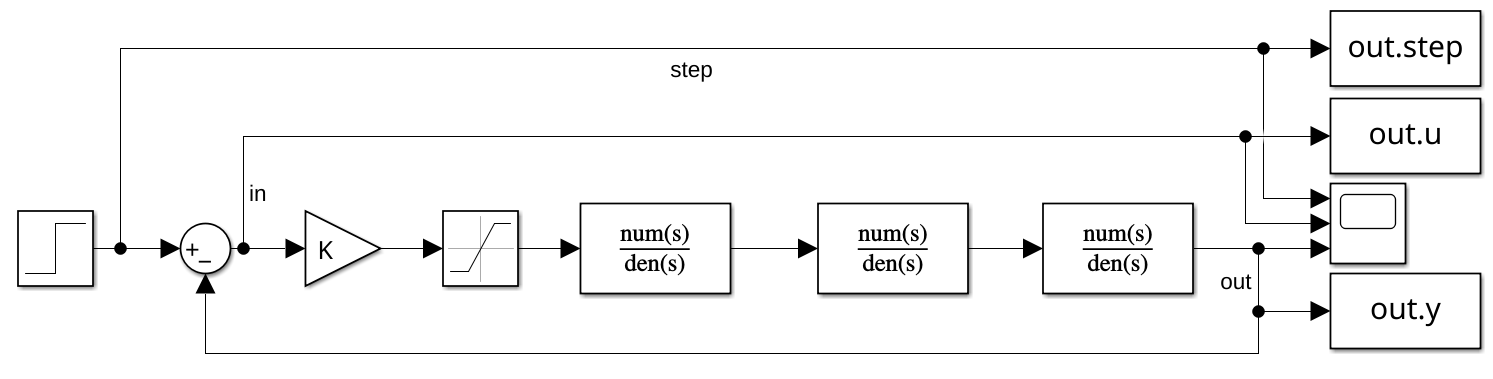
\includegraphics[width=0.9\textwidth]{graphix/2_a_b_c_model.png}
        \caption{Blockschaltbild (Screenshot aus \textit{Simulink})}
        \label{blockschaltbild_2abc}
    \end{figure}

    \begin{figure}[p]
        \centering
        \begin{subfigure}{\textwidth}
        \centering
                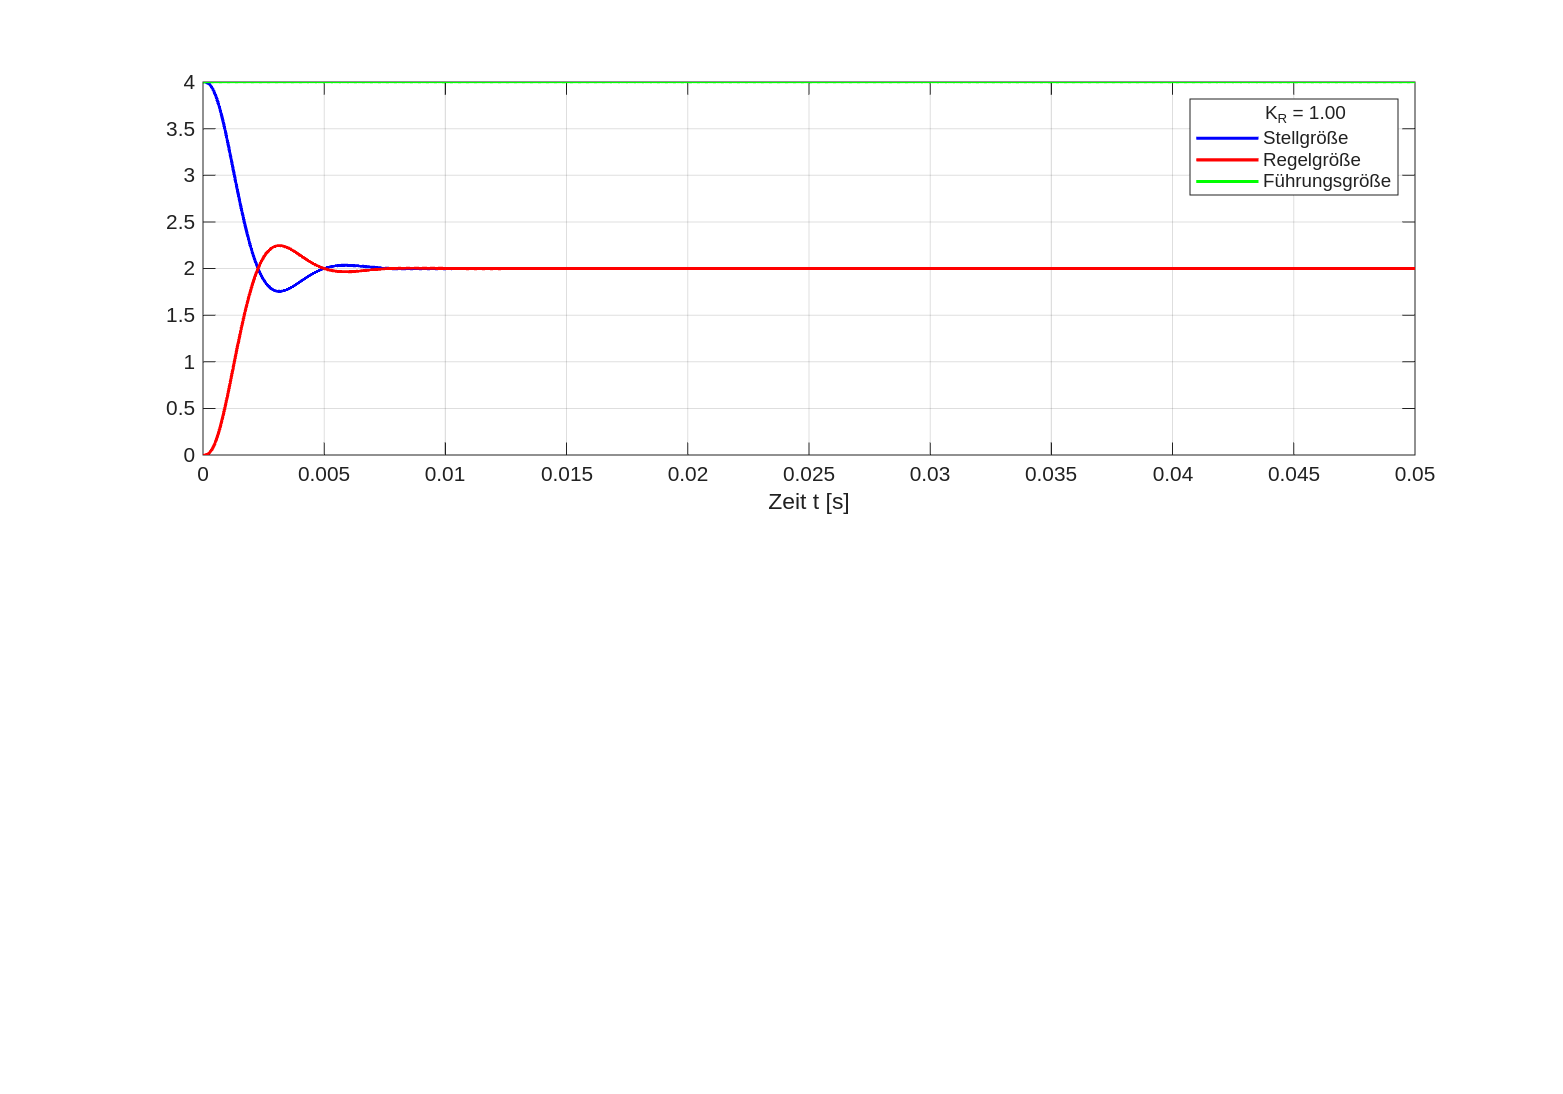
\includegraphics[trim=0cm 9cm 0cm 1cm, clip, width=0.9\textwidth]{graphix/P_Regler_K_1.00.png}
        \end{subfigure}
        
        \begin{subfigure}{\textwidth}
            \centering
            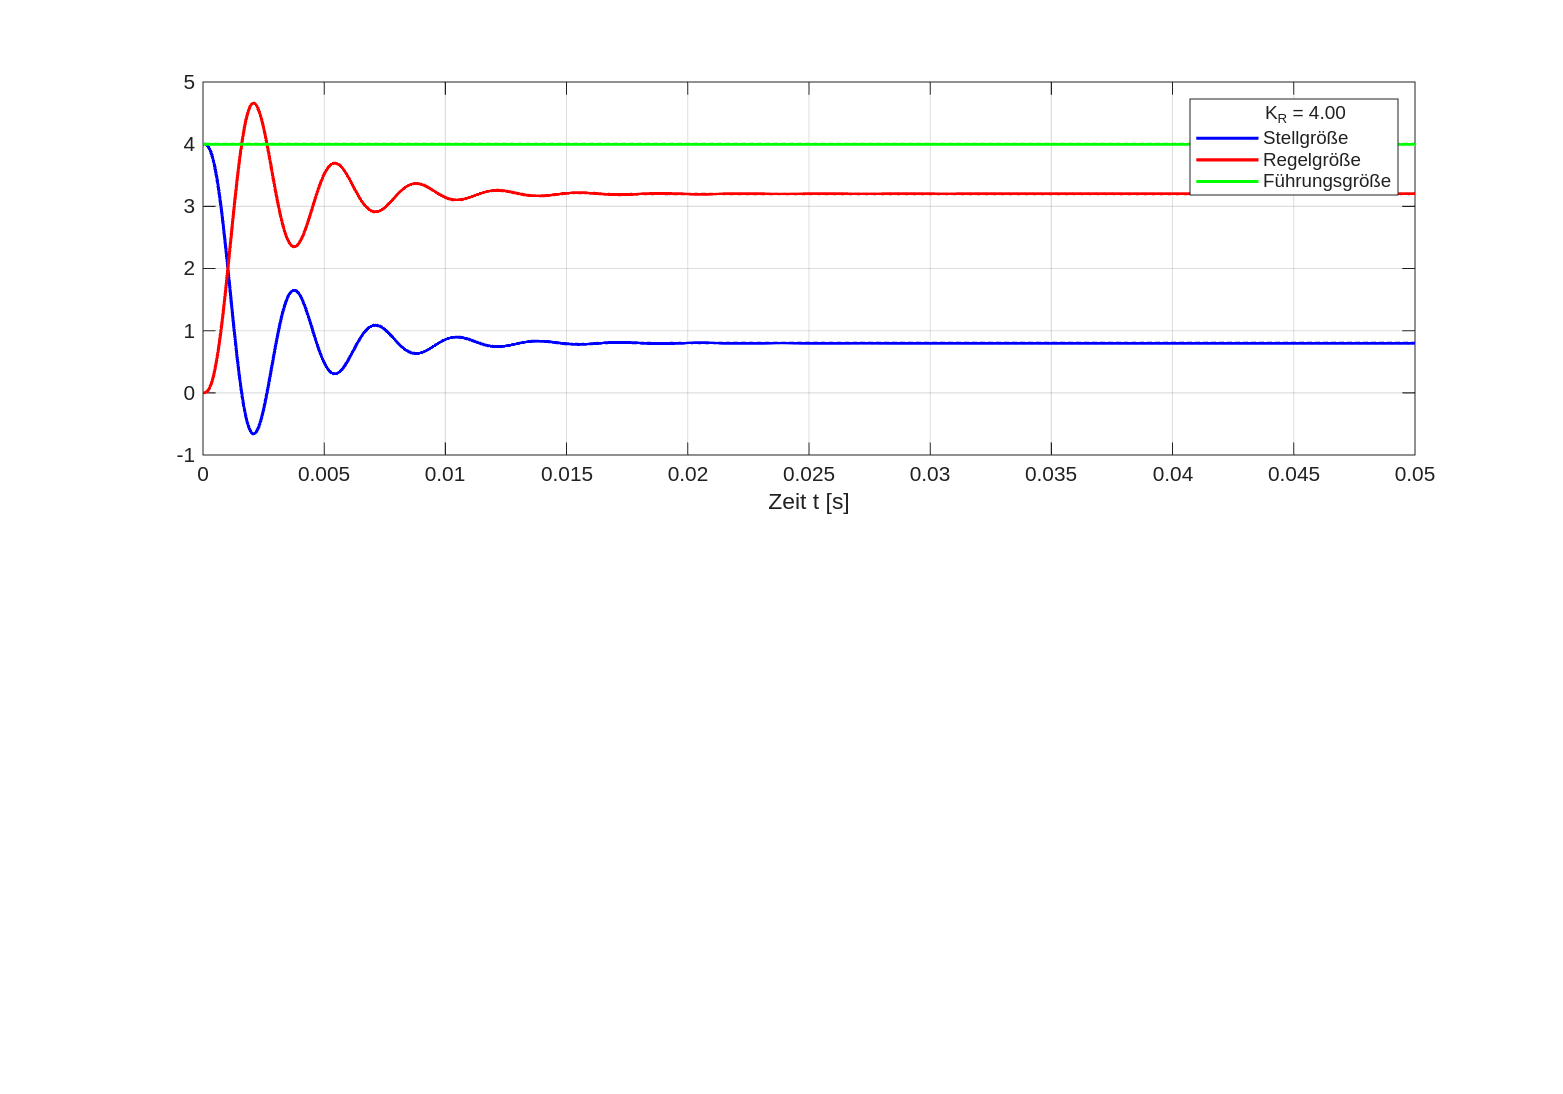
\includegraphics[trim=0cm 9cm 0cm 1cm, clip, width=0.9\textwidth]{graphix/P_Regler_K_4.00.png}
        \end{subfigure}
        
        \begin{subfigure}{\textwidth}
            \centering
            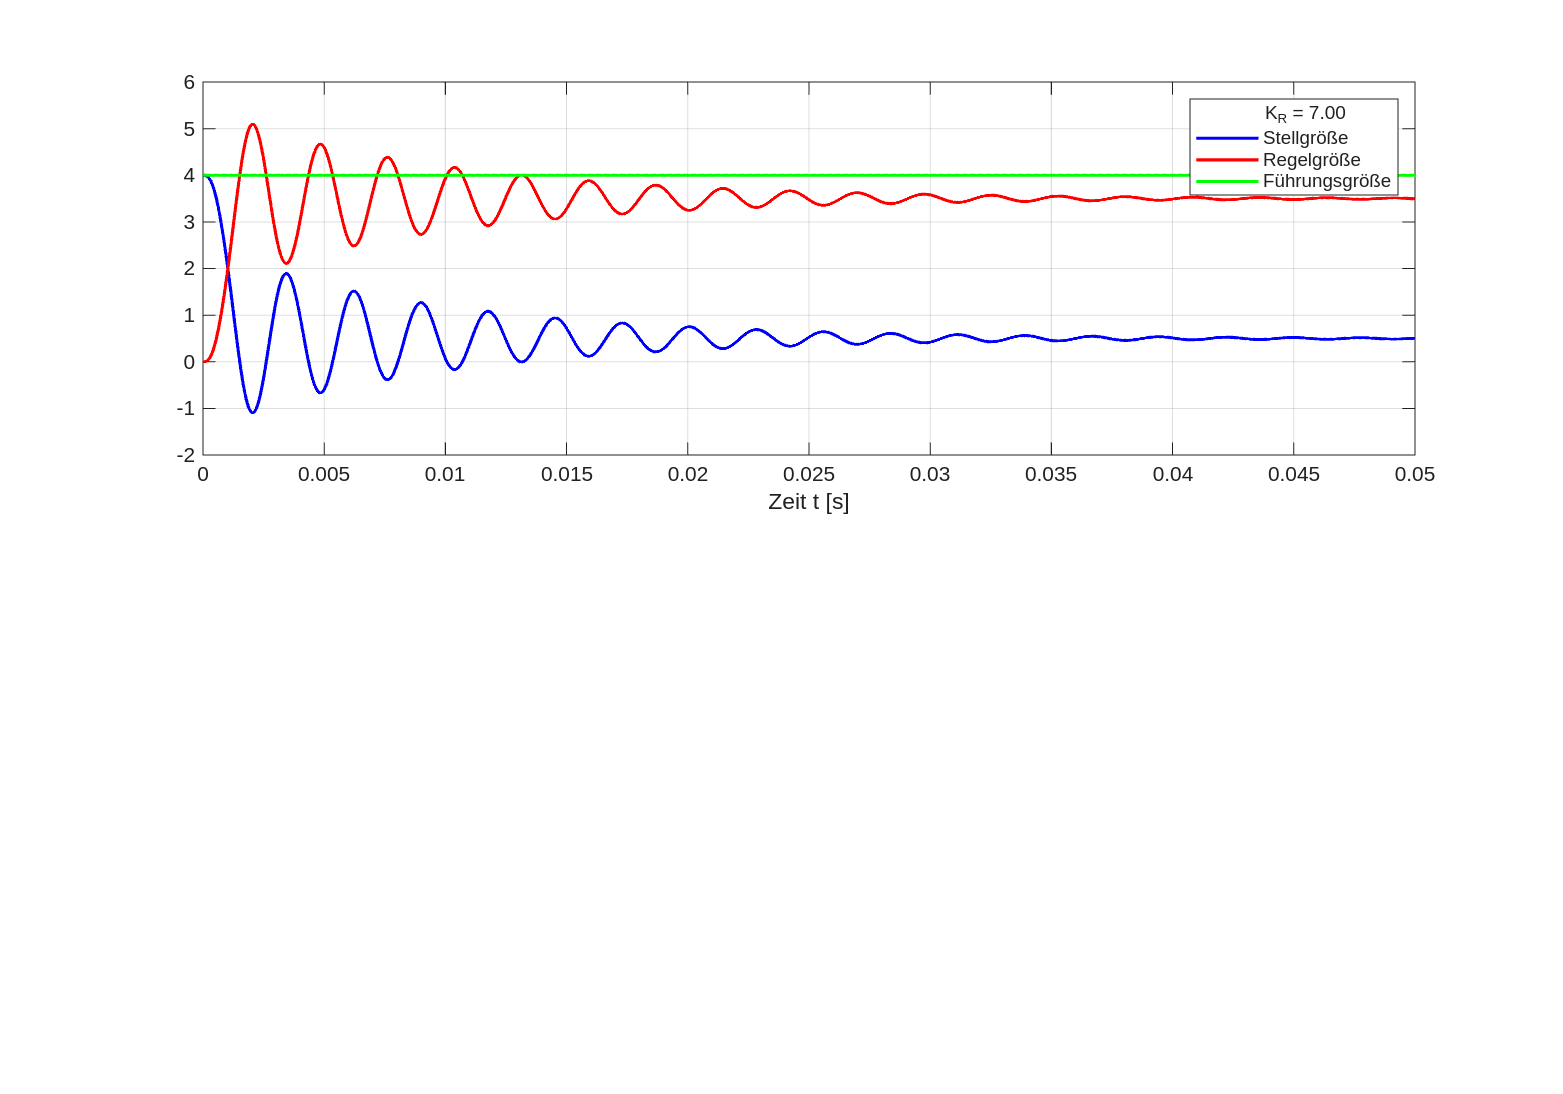
\includegraphics[trim=0cm 9cm 0cm 1cm, clip, width=0.9\textwidth]{graphix/P_Regler_K_7.00.png}
        \end{subfigure}
        
        \begin{subfigure}{\textwidth}
            \centering
            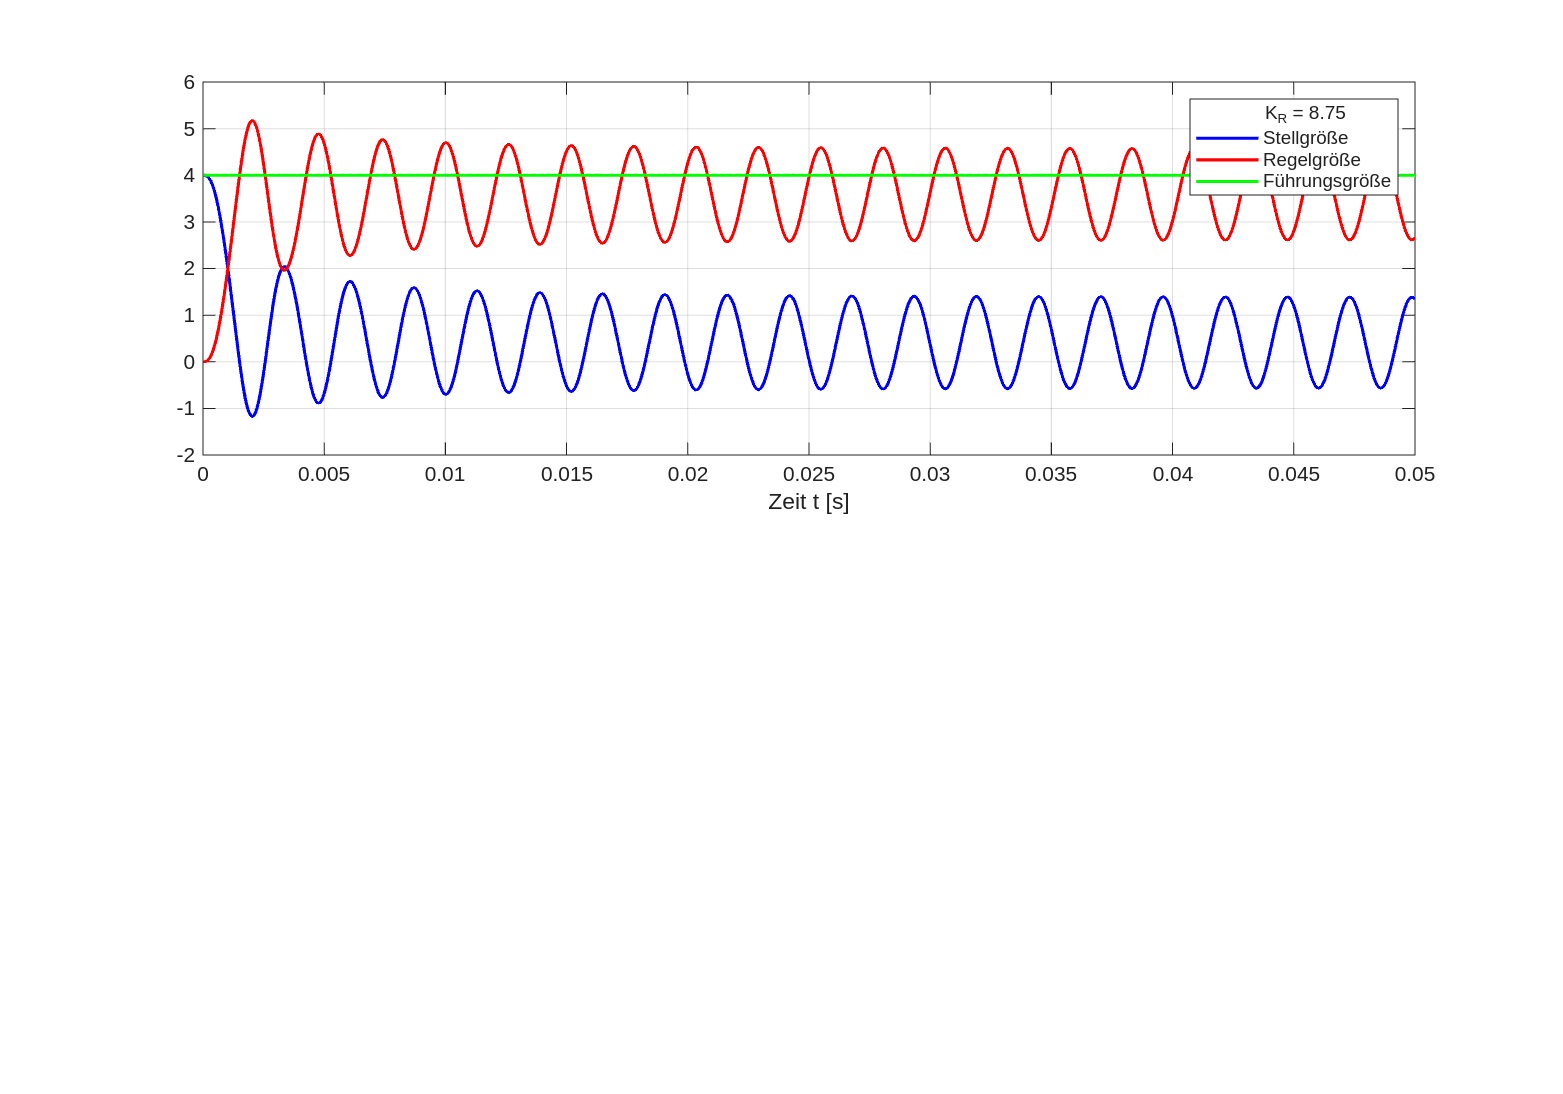
\includegraphics[trim=0cm 9cm 0cm 1cm, clip, width=0.9\textwidth]{graphix/P_Regler_K_8.75.png}
        \end{subfigure}
        
        \begin{subfigure}{\textwidth}
            \centering
            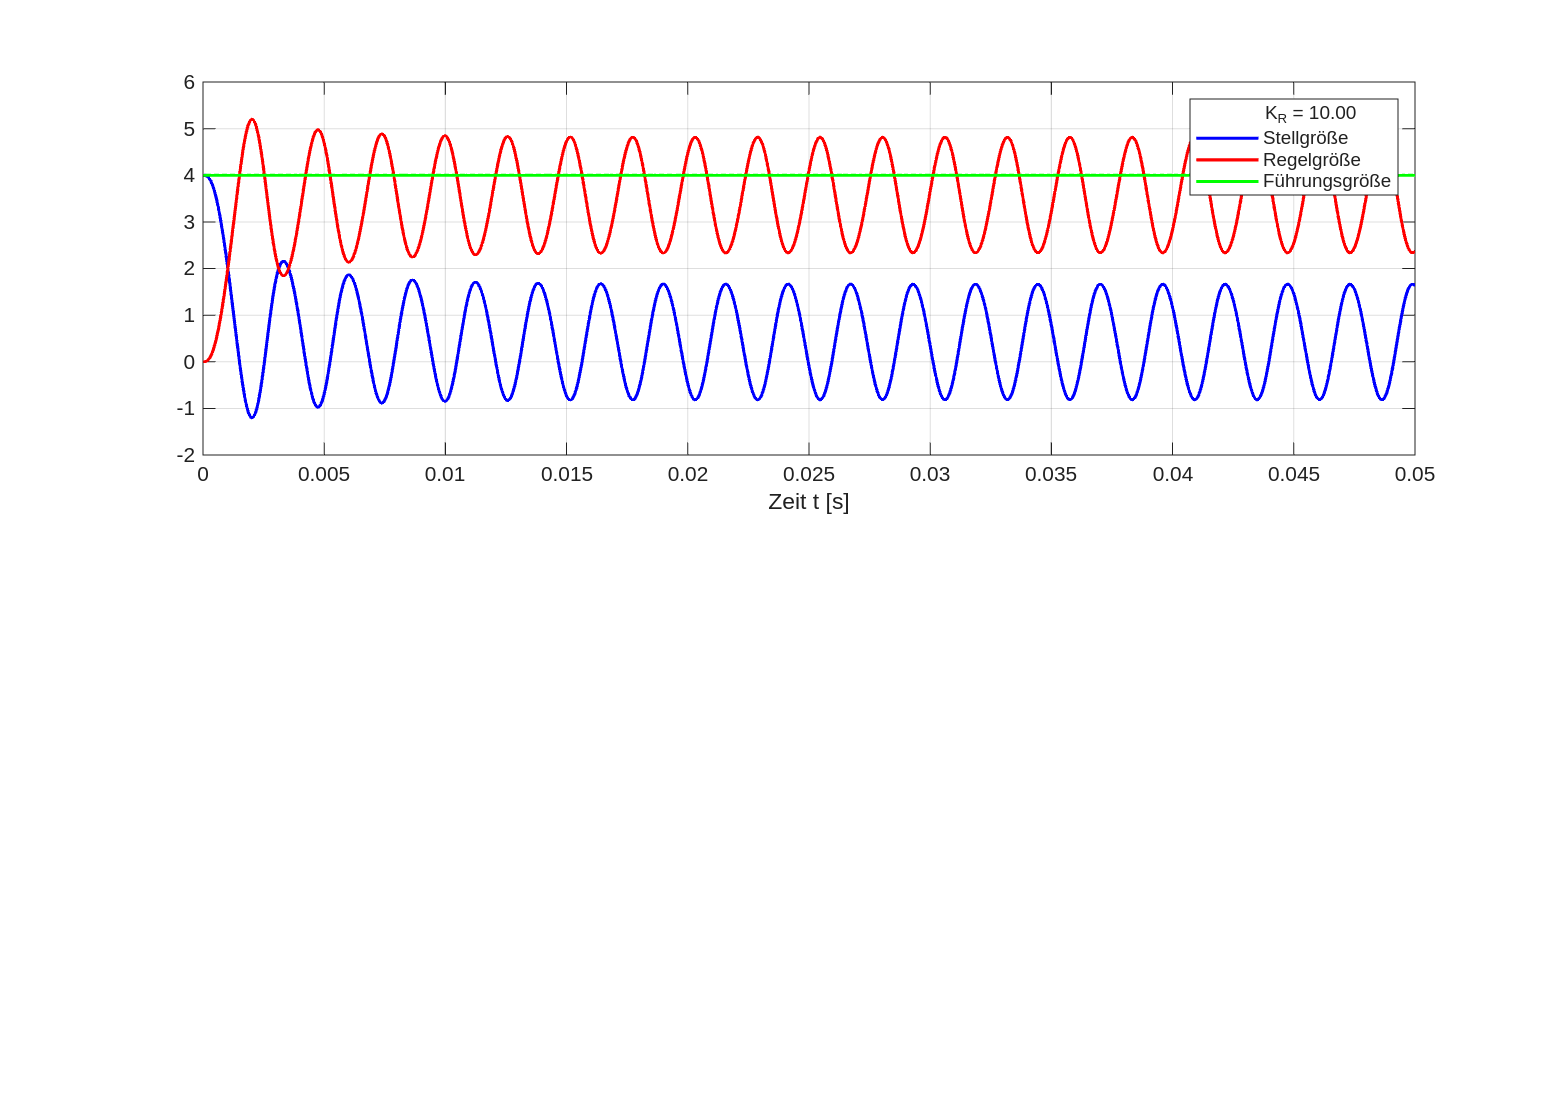
\includegraphics[trim=0cm 9cm 0cm 1cm, clip, width=0.9\textwidth]{graphix/P_Regler_K_10.00.png}
        \end{subfigure}
        
        \caption{\textit{Matlab}-Plots für verschiedene Reglerverstärkungen}
        \label{fig:2b_plots}
    \end{figure}

    \newpage
\subsection{Systemverhalten ohne Führungsgrößensprung}
    Dasselbe System wird nun ohne Führungsgrößensprung beobachtet: $w(t)=0$. Es wird der Fall des instabilen Systems mit $K_R=10$ betrachtet. Abbildung \ref{2_d_plot_w_0} zeigt die Signalverläufe. Ohne eine Erregung von außen (Führungsgrößensprung) oder von innen (Anfangsbedingungen ungleich Null) bleibt das System in Ruhe. Die Differenz am Summenpunkt ist immer Null. Deswegen werden Stell- und Regelgröße nie aktiv. Dieses Verhalten ist korrekt in einer idealen mathematischen Umgebung. In einem realen Regelkreis gibt es immer Rauschen aufgrund thermischer Unruhen und kleinerer Ungenauigkeiten. Ein reales instablies System würde durch diese Störungen sofort aufschwingen.  

    Um das reale System besser zu simulieren wird eine Rauschquelle als Störsignal eingefügt. Diese wird dem Signal am Ausgang der Regelstrecke überlagert, bevor dieses an den Eingang des Reglers rückgekoppelt wird. In \textit{Simulink} gibt es dafür den Block \textit{Uniform Random Number}. Das erweiterte Model ist in Abbildung \ref{blockschaltbild_2e} abgebildet. Das System schwingt auf. Es schwingt mit der Kreisfrequenz $\omega_R=2.549 krad/s $, welche fast gleich der Kreisfrequenz $\omega_{\pi}=2.449 krad/s$ ist. Die Abweichung beträgt nur $4\%$. Die Schwingung ist die physiklaische Antwort auf die Phasenverschiebung von $-180$ grad in der Strecke.  

    %d: w=0 ?
    \begin{figure}[H]
        \centering
        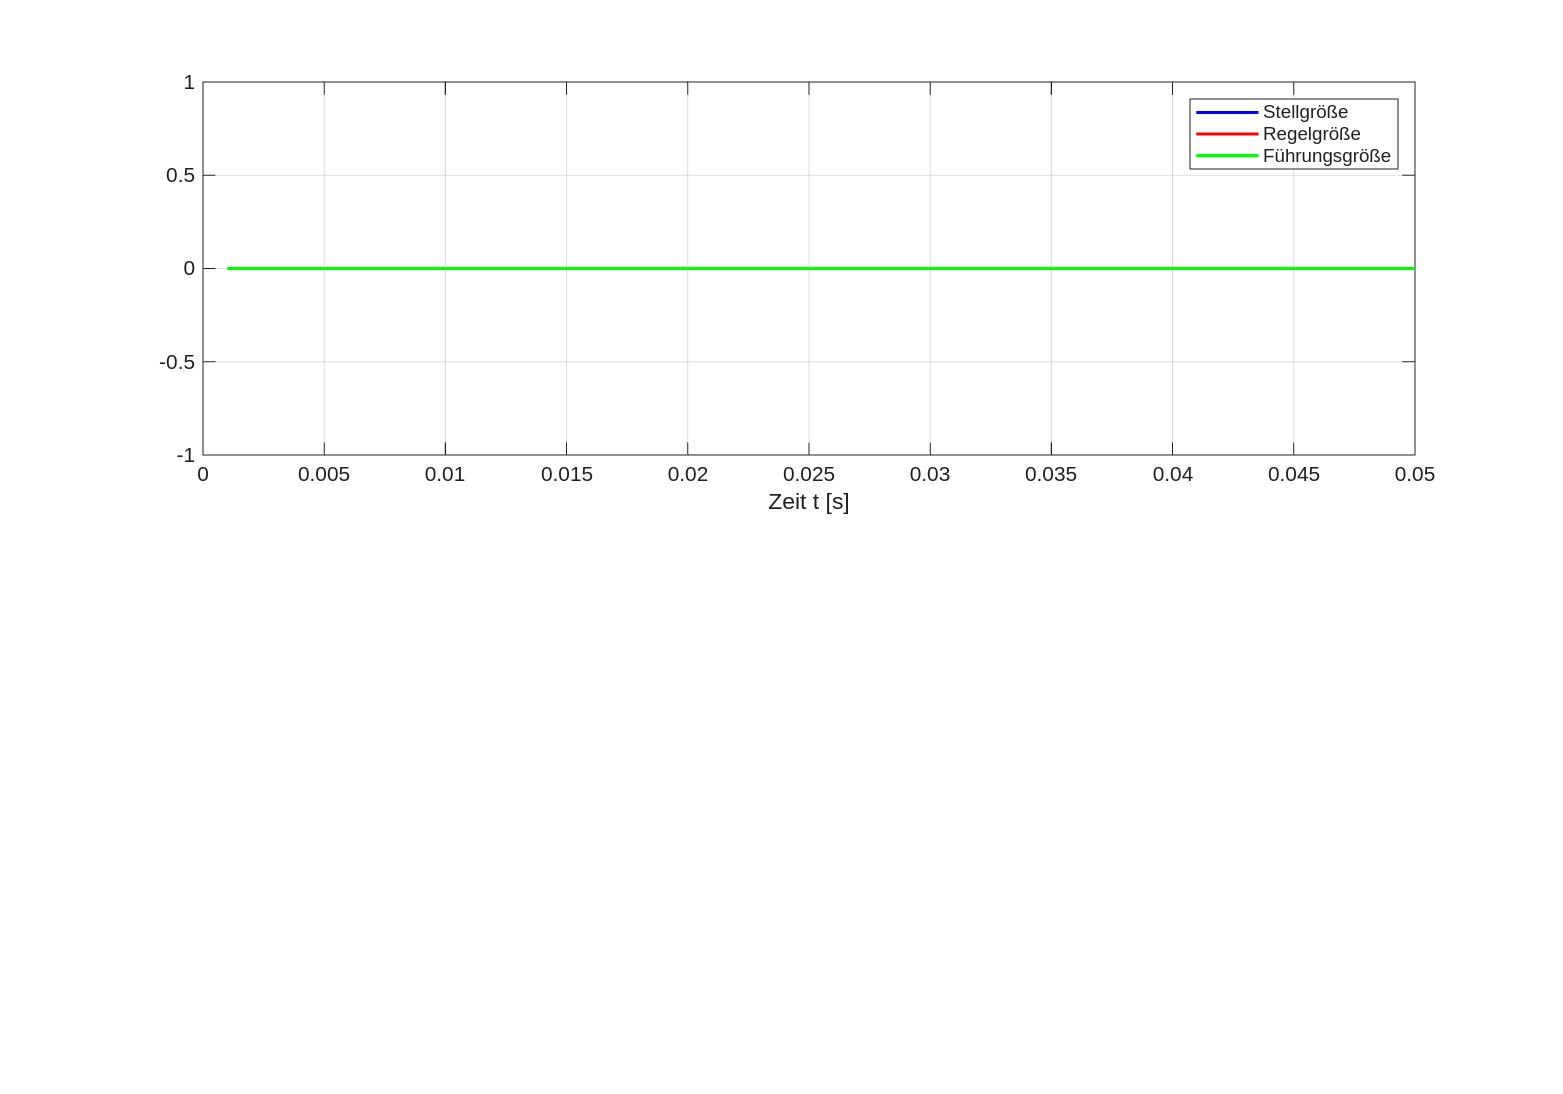
\includegraphics[trim=1.8cm 9.5cm 1.8cm 0.5cm, clip, width=\textwidth]{graphix/P_Regler_K_10.00_w_0.png}
        \caption{\textit{Matlab}-Plot für $w(t)=0$}
        \label{2_d_plot_w_0}
    \end{figure}

    %e: rauschquelle?
    \begin{figure}[H]
        \centering
        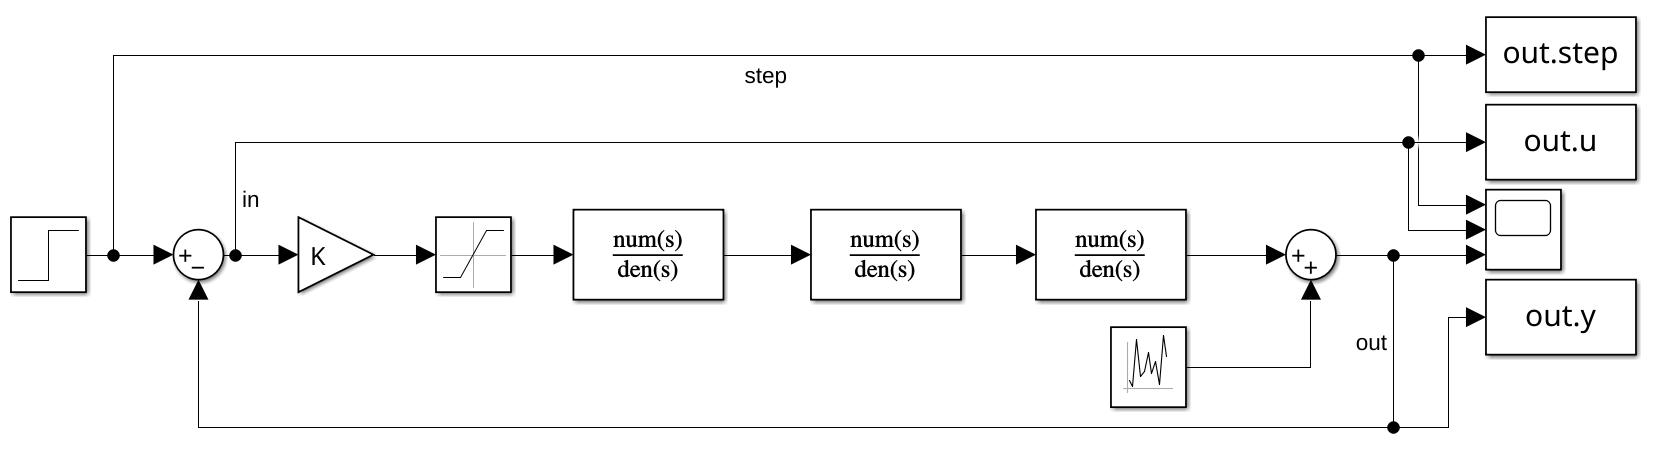
\includegraphics[width=0.9\textwidth]{graphix/2_e_model.png}
        \caption{Blockschaltbild (Screenshot aus \textit{Simulink})}
        \label{blockschaltbild_2e}
    \end{figure}

    \begin{figure}[H]
        \centering
        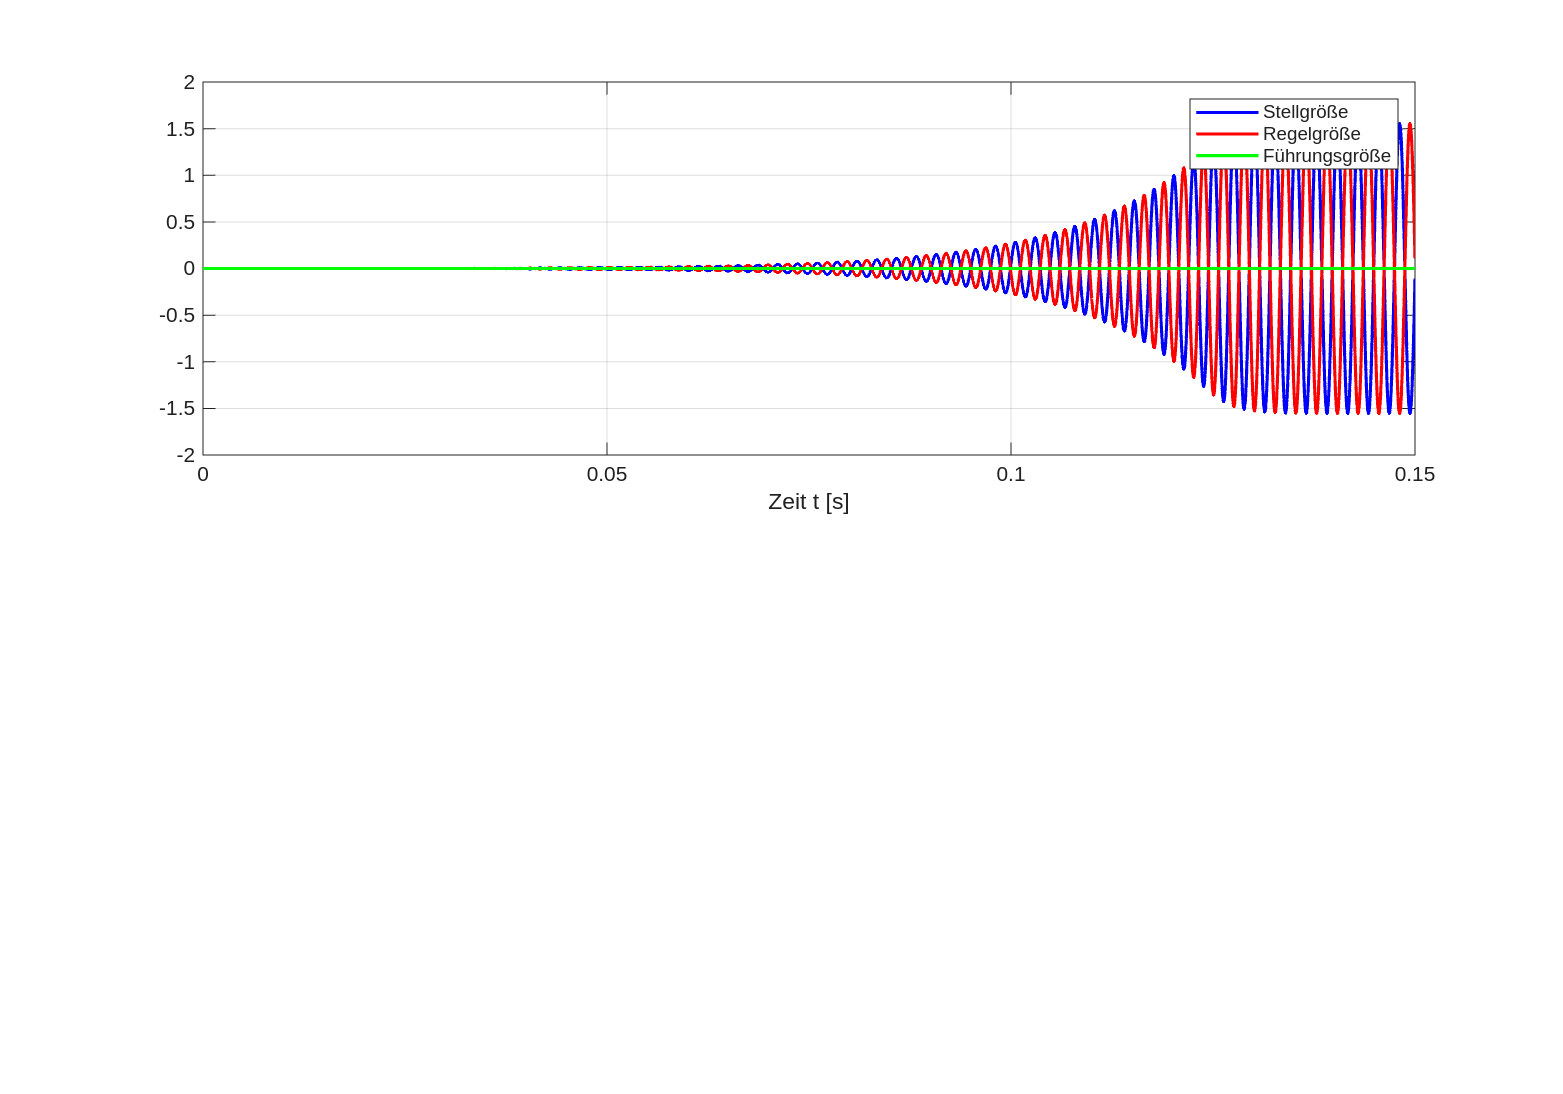
\includegraphics[trim=1.8cm 9.5cm 1.8cm 0.5cm, clip, width=\textwidth]{graphix/P_Regler_K_10.00_rauschen.png}
        \caption{\textit{Matlab}-Plot für $w(t)=0$ (mit Rauschquelle)}
        \label{2_e_plot_w_0_rauschquelle}
    \end{figure}

    %aus matlab: omega = 2549 rad/s